\chapter{Architecture}

In this chapter we present the overall architecture of the program, describe the individual components briefly and showcase some basic data-flow within the program. In the following chapters we focus on the main components and describe each in detail.

% explain that MainApplication is basically also a container, a single source of truth, that holds data that can be fetched from other components

% explain a simple data flow, use a similar example as from specification 3.3, but explain it in greater details, do not forget to mention that, e.g., side pane calls a draw method on the tools and they render "themselves"

\section{Architecture overview}

The following Figure \ref{fig:architecture} illustrates the main components in the architecture of the Pepr3D application. Each colour represents a separate component, while the arrows denote how data typically flow and how components usually communicate.

\vspace{20pt}

\begin{figure}[h]
	\centering
	\centerline{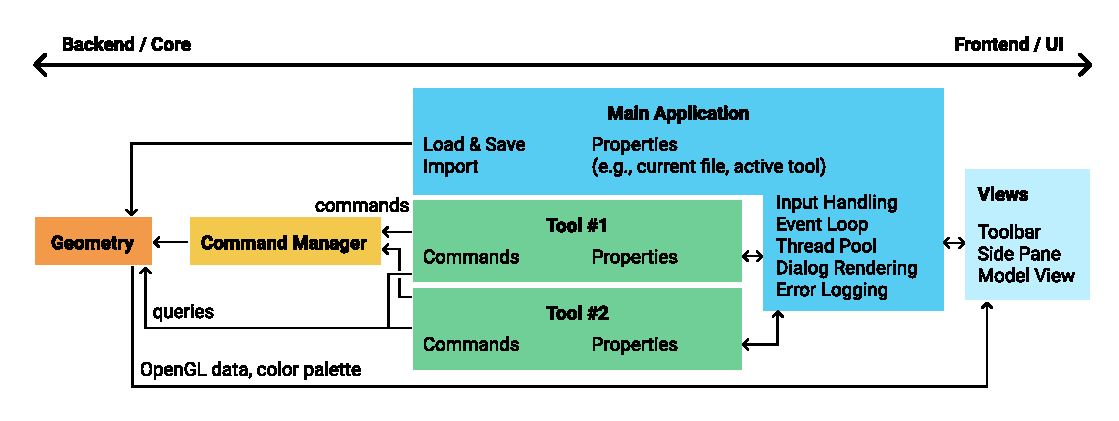
\includegraphics[scale=1.0]{images/diagram.eps}}
	\caption{An overview of the Pepr3D architecture.}
	\label{fig:architecture}
\end{figure}

\begin{itemize}
\item \textbf{Main Application} is the owner of the whole architecture. It contains functionality which is important for the whole application (like thread pooling or error logging) and owns and contains the other data structures. It acts as a single source of truth, holding the data that is valid at every moment (like the selected tool or the current model). This data is then fetched from the \texttt{MainApplication} by other components.

\item \textbf{Views} are the elements that fill the screen of the application. They handle rendering the user interface and allowing the user to perform basic actions to handle Pepr3D like rotating and zooming in on the model in \texttt{ModelView}, choosing a tool from the \texttt{Toolbar} or changing the tool's properties in \texttt{SidePane}.

\item \textbf{Tools} are the components that allow the user to interact with the data. Each tool has its properties that can be changed by the user via the user interface. If the user wishes to perform an action that would change the geometry (like colouring a triangle), the tool invokes a command which will take care of the action. The tool specifies how the right panel (\texttt{SidePane}) will look for each tool and can also query the \texttt{Geometry} class for simple information like the hovered triangle id.

\item \textbf{Command Manager and Commands} are the way Pepr3D handles the \textit{Undo} and \textit{Redo} operations. A \texttt{Command} is a single operation that can be ran by the \texttt{CommandManager} or joined with other \texttt{Command}s. A simple example of a command is the \texttt{PaintSingleColor} command. It takes a list of triangle ids and a color, and simply changes the color of those triangles to the new color. It can be joined with other \texttt{PaintSingleColor} commands, which have the same color by merging the two triangle id lists. The \texttt{CommandManager} then holds the stack of applied commands, saves the snapshots of the current geometry and is able to recreate any state by reverting to the older snapshots and running the commands again.

\item \textbf{Geometry} is the main data structure of the application. It holds the data of the triangles, their colors, normals, etc. It also generates the buffers for OpenGL and provides an API for the Commands (for non-\texttt{const} purposes) and Tools (for \texttt{const} purposes such as finding the hovered triangle id).
\end{itemize}

The arrows between these components show the typical directions of communication. We can see, for example, that only \texttt{CommandManager} and the \texttt{MainApplication} send data to \texttt{Geometry}, while the user interface does not know anything about the \texttt{CommandManager}. Not every single communication is represented here, as for example certain Tools need read-only access to Geometry.

During the development we tried to separate the components as much as possible. Since our application is pretty basic, the pipeline is still connected quite a lot. We hope that this design is extendible though, and if the need arises, new components can be easily inserted into the overall architecture as illustrated in Figure \ref{fig:architecture}.

\section{Data flow}

In this section we demonstrate the data flow on a simple chain of operations an average user might perform. The sequence is the following and can be executed any time after launching the application: \textit{Import a model} $\rightarrow$ \textit{Select Bucket Painter tool} $\rightarrow$ \textit{Change settings on Bucket Painter} $\rightarrow$ \textit{Paint with the Bucket Painter} $\rightarrow$ \textit{Undo the operation}.

\begin{enumerate}
\item \textbf{Importing a model} causes the \texttt{MainApplication} to launch an asynchronous function that loads the new model, calculates the data for both the \texttt{MainApplication} and \texttt{Geometry} objects. This information includes the data structures for geometry operations or the calculations to re-orient the model correctly in the \texttt{ModelView}. After this step is done, \texttt{MainApplication} gets updated and holds the new \texttt{Geometry} object, which changes the geometry.

\item \textbf{Selecting the Bucket Painter} is, according to Figure \ref{fig:architecture}, a change of the \texttt{MainApplication}'s property. This is done via the \texttt{Toolbar} view. Upon selecting the new tool, when the next frame starts rendering, the \texttt{SidePane} will query the \texttt{MainApplication} object for the current tool, which will be the Bucket Painter. The \texttt{SidePane} will then let the Bucket Painter render its own settings within the \texttt{SidePane}.

\item \textbf{Changing Bucket Painter's settings} is changing the tool's properties. It is done within the \texttt{SidePane} view, which the Bucket Painter fills with relevant UI widgets (buttons, checkboxes, etc.). Changing these widgets will change the Bucket Painter's properties.

\item \textbf{Painting with Bucket Painter} by clicking on a certain triangle of the model. By clicking into the model view, an event gets created. The event is first processed in the \texttt{MainApplication} (e.g. if it is a \textit{drag and drop} event), then gets evaluated in \texttt{ModelView} (e.g. if it is a right click to rotate the view) and the \texttt{ModelView} then passes it into the tool, if it is required. The Bucket Painter gets the left click, queries the \texttt{Geometry} for the hovered triangle id, queries the \texttt{Geometry} again for the bucket spread and then executes a \texttt{PaintSingleColor} command. This command gets enqueued into the \texttt{CommandManager}, which executes it, changing the \texttt{Geometry}. In the next rendering frame, the \texttt{ModelView} notices, that the OpenGL geometry buffers are dirty, asks the \texttt{Geometry} to recalculate the buffers and renders the new colors.

\item \textbf{Undoing the last command} by clicking the \textit{Undo} button invokes the \texttt{CommandManager}. It restores the last snapshot of the \texttt{Geometry}, then re-runs all commands except the last one and updates the \texttt{Geometry}. This effectively restores the state before clicking with the Bucket Painter.
\end{enumerate}

This simple sequence of operations describes the majority of the program runtime data flow and control handling. It highlights important concepts of the UI -- such as the tool's user interface being rendered by the tool itself or the \texttt{CommandManager} semantics.